\documentclass{article}
\usepackage[12pt]{extsizes}
\usepackage[T2A]{fontenc}
\usepackage[utf8]{inputenc}
\usepackage[english, russian]{babel}

\usepackage{amssymb}
\usepackage{amsfonts}
\usepackage{amsmath}
\usepackage{enumitem}
\usepackage{graphics}
\usepackage[dvips]{graphicx}
\graphicspath{{images/}}

\usepackage{lipsum}



\usepackage{geometry} % Меняем поля страницы
\geometry{left=1cm}% левое поле
\geometry{right=1cm}% правое поле
\geometry{top=1.5cm}% верхнее поле
\geometry{bottom=1cm}% нижнее поле


\usepackage{fancyhdr} % Headers and footers
\pagestyle{fancy} % All pages have headers and footers
\fancyhead{} % Blank out the default header
\fancyfoot{} % Blank out the default footer
\fancyhead[L]{Математика}
\fancyhead[C]{\textit{Геометрия}}
\fancyhead[R]{29 сентября 2022}% Custom header text


%----------------------------------------------------------------------------------------

%\begin{document}\normalsize
\begin{document}\large


\begin{center}
\textbf{Клетчатая бумага}
\end{center}

\begin{figure}[h]
	\begin{center}
		\begin{minipage}[h]{0.3\linewidth}
			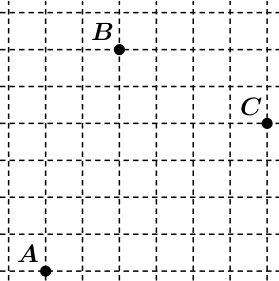
\includegraphics[width=1\linewidth]{1.png}
			\caption{Задача 1} %% подпись к рисунку
			\label{ris:1} %% метка рисунка для ссылки на него
		\end{minipage}
		\hfill 
		\begin{minipage}[h]{0.3\linewidth}
			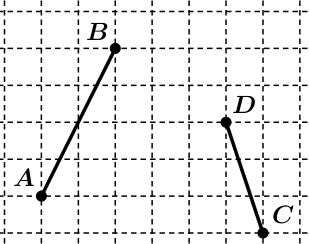
\includegraphics[width=1\linewidth]{5.png}
			\caption{Задача 5} %% подпись к рисунку
			\label{ris:5} %% метка рисунка для ссылки на него
		\end{minipage}
	\hfill 
		\begin{minipage}[h]{0.3\linewidth}
			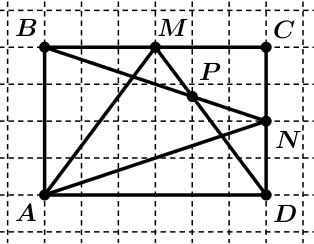
\includegraphics[width=1\linewidth]{6.png}
			\caption{Задача 6} %% подпись к рисунку
			\label{ris:6} %% метка рисунка для ссылки на него
		\end{minipage}
	\end{center}
\end{figure}

\begin{enumerate}[label*=\protect\fbox{\arabic{enumi}}]

\item Постройте центр описанной окружности треугольника $ABC$

\item Постройте какой-нибудь треугольник, две медианы которого перпендикулярны.

\item Отметьте на клетчатой бумаге 12 точек, лежащих на одной окружности.

\item На клетчатой бумаге в узлах сетки отмечено 20 точек, лежащих на одной окружности. Какого радиуса может быть эта окружность?

\item Найдите угол между прямыми $AB$ и $CD$

\item Докажите, что углы $MAN$ и $BPM$ равны.

\item В прямоугольном треугольнике $ABC$ с катетами 1 и 3 больший катет $AB$ разделили на 3 равных отрезочка $AD$, $DE$, $EB$. Найдите сумму углов $\angle CAD + \angle CDE + \angle CEB$

\end{enumerate}
\end{document}